\bluepage{Compute Shaders}

\begin{frame}
\frametitle{Compute Shader}
	\begin{itemize}
	\item Compute shader is located outside of common rendering pipeline.
  \item Compute shader can be used for general computing - GPGPU (other shader are in some way restricted).
  \item Compute shader share syntax with the rest of shader and can be used on different platforms.
	\end{itemize}
	\begin{figure}[h]
	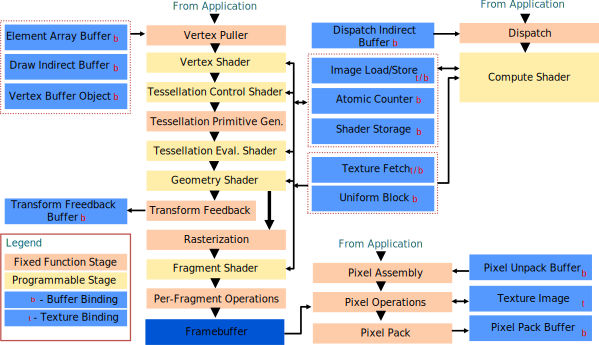
\includegraphics[width=10cm,keepaspectratio]{pics/opengl43.pdf}
	\end{figure}
\end{frame}

\begin{frame}
\frametitle{Compute Shader}
	\begin{figure}[h]
	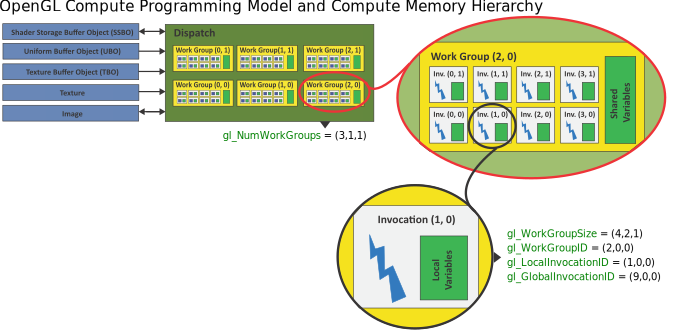
\includegraphics[width=11cm,keepaspectratio]{pics/compute.pdf}
	\end{figure}
\end{frame}

\begin{frame}[fragile]
\frametitle{Compute Shader - example}
{\scriptsize
\begin{minted}[bgcolor=bg]{packages/graphics.py:GLShaderLexer -x}
#version 430

layout(binding=0)buffer Input{vec4 i[];};//input buffer
layout(binding=1)buffer Output{vec4 o[];};//output buffer
layout(local_size_x=32,local_size_y=1,local_size_z=1)in;//work-group size

uniform uint num;//number of elements in buffers

void main(){
  //gl_GlobalInvocationID = gl_WorkGroupID*gl_WorkGroupSize + gl_LocalInvocationID	
  uint gid = gl_GlobalInvocationID.x;
  if(gid >= num)return;
  vec3 v = i[gid].xyz;
  o[gid] = vec4(normalize(v),length(v));
}
\end{minted}
}
\end{frame}

\begin{frame}[fragile]
\frametitle{Compute Shader - example}
{\scriptsize
\begin{minted}[bgcolor=bg]{packages/c_cpp.py:CppLexer -x}
uint32_t num=100;
GLuint CompBufferInput;
glCreateBuffers(1,&CompBufferInput);
glNamedBufferData(CompBufferInput,sizeof(float)*4*num,nullptr,GL_STATIC_DRAW);

GLuint CompBufferOutput;
glCreateBuffers(1,&CompBufferOutput);
glNamedBufferData(CompBufferOutput,sizeof(float)*4*num,nullptr,GL_DYNAMIC_COPY);

glBindBufferBase(GL_SHADER_STORAGE_BUFFER,0,CompBufferInput);
glBindBufferBase(GL_SHADER_STORAGE_BUFFER,1,CompBufferOutput);

glUseProgram(ComputeShader);
glUniform1ui(glGetUniformLocation(ComputeShader,"num"),num);

uint32_t workGroupSize = 32;

glDispatchCompute(divRoundUp(num,workGroupSize),1,1);
\end{minted}
}
\end{frame}

\begin{frame}[fragile]
\frametitle{Compute Shader - dispatch synchronization}
  \begin{itemize}
    \item Synchronization needs to be done between two shaders thats operates on same data.
    \item Synchronization is performed using glMemoryBarrier(); command.
  \end{itemize}

{\scriptsize
\begin{minted}[bgcolor=bg]{packages/c_cpp.py:CppLexer -x}
//This compute shader creates buffer with vertices.
glDispatchCompute(
    this->TileCount[(this->NumLevels-2)*2+0],
    this->TileCount[(this->NumLevels-2)*2+1],
    1);

//Wait for modification to SSBO
glMemoryBarrier(GL_SHADER_STORAGE_BARRIER_BIT);

//Draw generated vertices
glDrawArrays(...)
\end{minted}
}
\end{frame}

\begin{frame}[fragile]
\frametitle{Compute Shader - thread synchronization}
  \begin{itemize}
    \item Threads in work-group are execute in warp/wavefronts.
    \item We can synchronize threads that are part of work-group.
    \item We cannot synchronize threads that are part of different work-groups.
    \item Threads that are part of warp do not have to be synchronized.
    \item Synchronization is performed by barrier() command.
    \item A barrier command has to lie on program path that can be access by all threads in work-group.
    \item A barrier command stops every thread until all other threads in work-group reach it.
  \end{itemize}
  Example:
{\scriptsize
\begin{minted}[bgcolor=bg]{packages/graphics.py:GLShaderLexer -x}
layout(std430,binding=0)readonly buffer SFData{float data[];};
shared float array[size];
void main(){
  //cooperative reading from global memory into local/shared memory.
  array[gl_LocalInvocationID.x]=data[gl_GlobalInvocationID.x];
  //wait for all threads
  barrier();
  //...
}
\end{minted}
}
\end{frame}

